\begin{introduction}
\section{Introduction}
Temporal networks are prevalent across many systems in the modern world, be it natural, social, technological, financial or industrial. A few examples of temporal networks include public transport\cite{transport_example}, human interaction\cite{social_example}, stock markets\cite{stocks_example} and wireless sensors\cite{wireless_example}. These examples show that a diverse amount of systems can be modelled as a temporal network, or are inherently so. The analysis of such networks can yield new and useful information that was previously not obvious from the raw data (for example, message logs). A convenient library which allows for such network modelling and analysis would prove very useful for multiple disciplines and domains.

A static network can be represented as a graph, consisting of nodes and edges. In its simplest form, a graph is a set of points interconnected with lines, where each line connects a pair of points. The graph connectivity is defined in the incidence function, which associates edges and node pairs (ch01 \cite{graph_theory}). Mathematically, a graph G is an ordered triple of nodes, edges and the incidence function:

\begin{minipage}{0.4\textwidth}
    \begin{flushleft}
    \[ G = (V, E, \psi) \]
    \end{flushleft}
\end{minipage}
~
\begin{minipage}{0.4\textwidth}
    \begin{flushright}
    \[ V = (a, b, c) \]
    \[ E = (x, y, z) \]\
    \[ \psi(x) = (ab),\ \psi(y) = (ac),\ \psi(z) = (bc) \]
    \end{flushright}
\end{minipage}\\[0.25cm]
A graph may be undirected, where an edge z connecting nodes b and c does not specify a direction, meaning the edge is valid for both directions bc and cb. Conversely, a directed graph (digraph) has directional edges. Like the undirected graph, the incidence function describes the relationship between edge and nodes;
\[ \psi(xy) = (x, y) \]
where edge xy connects nodes x and y, with node x being the source and node y the sink (ch10 \cite{graph_theory}). The edges of the graph can hold information (such as weights) that describe the relationship/connections between nodes. Such a graph is known as a labelled graph. It is important to note that modelling a temporal network is fundamentally different from a static network, i.e. you cannot simply generalize a concept/model based on a static network into a temporal one (s2.1 \cite{temporal_theory}).

In a temporal graph, each edge has a label which indicates some measure of time (discrete or continuous). This could be the start time(s) of when the edge is active, along with a duration of how long the edge is active. A temporal graph can be described as a graph whose connections change over time. The nodes of the graph remain static, while the edges update as time changes. A temporal graph can also be perceived as sequence of static graphs with an (unchanging) set of nodes. Other edge labels could correspond to temporal information if interpreted correctly (s2 \cite{intro_temporal}).
In the discrete time case, the temporal graph can be presented as a static graph $G=(V, E)$ with each edge labelled with a list of natural numbers corresponding to when that edge is active (figure 1). This time-edge (or contact/link) triple $e = (i, j, t)$ of source, sink and active time are the fundamental building blocks of temporal graphs.
\clearpage
\begin{figure}
    \centering
    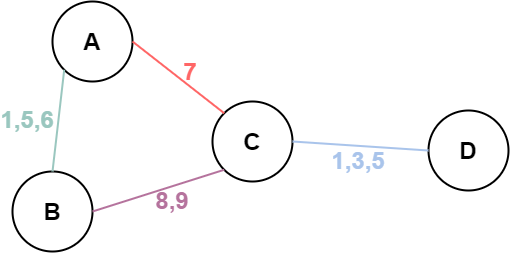
\includegraphics[scale=0.5]{images/temporal_graph_a.png}
    \caption{An static graph illustration of a temporal network.}
\end{figure}
\begin{figure}
    \centering
    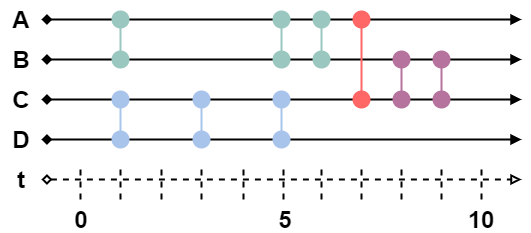
\includegraphics[scale=0.6]{images/temporal_graph_b.png}
    \caption{An timeline illustration of a temporal network.}
\end{figure}
The above figures illustrate a temporal network in two representations. The first figure is a static graph, with each edge labelled with the active/available times (time-edges/links). The second figure shows the timeline of the network, with the times-edges become available represented as connections between the node rows. The timeline representation better illustrates the temporal connectivity of the graph, while the static representation shows the structure of the network. Note that in the static graph, while node D is 'connected' to node A,B through C, it is in fact not possible to traverse from A/B to D, as the time-edges from C to D are, in a sense, too early. This indicates the lack of temporal information/intuition a static representation has, and further indicates that static and temporal networks are indeed fundamentally distinct.
Once a temporal graph is built, there are many measurements and algorithms that can be applied to the network in order to produce temporal metrics. Network latency, reachability and centrality are all distinctive properties of temporal networks, and can have a large impact on the performance of the network being modelled.\\
The research and interest in the domain of temporal networks is increasing as technology advances, and there is growing evidence \cite{social_metrics} that the modelling and analysis of such networks can produce useful results and information. Therefore, a convenient and purposeful library to enable this effort would be advantageous.
\end{introduction}
\vspace{1cm}
\clearpage